%% Einleitung.tex
%% $Id: einleitung.tex 28 2007-01-18 16:31:32Z bless $
%%

\chapter{Introduction}
\label{ch:Introduction}
%% ==============================
% CLEARLY SHOW CONTRIBUTIONS AND LINK THEM TO SECTIONS

%\section{Background}

\section{Motivation}

\begin{comment}
\textcolor{red}{To Edit}

Over the last several years, accessibility is becoming a word with ever increasing importance. Over the last several decades several nations have passed regulatory acts which guarantee equal treatment between all people\cite{webaim}. For example, in 1994 Germany passed the Accessibility Ordinance (Behindertengleichstellungsgesetz) which meant that no one can be disadvantaged due to their disability.

As a result of the regulatory acts in many nations it was required to have documents being able to be read by everyone. Everyone is supposed to have access to documents.

Making accessible documents in paper form is difficult, because each group needs to have its document printed separately. Blind people need to have documents printed in braille, which requires special equipment. Furthermore it is very heavy. Visually impaired people have document requirement which person to person, so it is very difficult to prepare printed documents for them.

Making documents accessible in electronic form is much easier, as the document can be adjusted to each group's requirements easily. The output is also adjustable so if a blind person prefers using a screen reader to a refreshable braille display they are free to do so with little to no extra effort. Visually impaired people can change font, size and colors with only a few clicks.

Currently, the dominant format for electronic documents are PDFs (Portable Document Format, extension \lstinline{.pdf}) and word documents(extensions \lstinline{.doc}, \lstinline{.docx}, \lstinline{.odt}). While PDF/UA (PDF/Universal Accessibility) has done much in terms of accessibility, there are still some shortcomings. First of all both formats have a predefined page size. While this is useful for printed documents, a computer screen can rarely display all contents of the document to the detriment of visually impaired people.\cite{EPUBzone} The font size is also predetermined and cannot be changed. While zooming can increase the apparent size of the font, the document width may not fit the screen. Furthermore semantic information normally is missing from the documents. For example, a PDF does not necessarily have the document language defined. A PDF might also not have a predefined reading order which means that the header and footer might be output by the screen reader every page. 

Conversely, this means that an electronic document format with no set document size, containing semantic and structure information and a set reading order would be better suited to meet the demands of accessibility. 

\textcolor{red}{To Edit End}

\end{comment}

In recent years, the topic of accessibility has become increasingly important, especially for accessible documents. Several states have passed regulatory laws that ensure equal treatment of all people and ensure that documents are accessible to all \cite{webaim}.\\
The currently dominant format for accessible electronic documents are Microsoft Word and PDF (Portable Document Format) documents, or more precisely PDF/UA (PDF/Universal Accessibility) documents. First of all, both formats have a predefined page size. While this is useful for printed documents, a computer screen can rarely display all contents of the document to the detriment of visually impaired people \cite{EPUBzone}. Therefore, an electronic document format without a fixed document size containing semantic and structural information and a fixed reading order would be better suited to meet the requirements of accessibility.\\
Furthermore, different "selectable" forms of presentation would be advantageous, especially for graphics or mathematical formulas. For example, formulas in the \LaTeX $\mbox{ }$ source code for blind users or high-contrast images for users with limited residual vision. This could be combined with EPUB 3 \cite{EPUBzone}.


EPUB stands for {\bf E}lectronic {\bf PUB}lication and is a format primarily used for books in an electronic format (E-book). The EPUB format was created by the International Digital Publishing Forum (IDPF) and the current version is 3.1 which is a minor update to EPUB 3 \cite{EPUBspecs}. EPUB uses XML based formats like XHTML, and thus also uses the accessibility standards and guidelines already established in many nations like the Web Content Accessibility Guidelines (WCAG)\cite{WCAG}. This was done as reading systems can have different screen sizes and the EPUB content can therefore be reflowable. Font type and size can also be adapted to the individual needs of the users. Visually impaired people could therefore adjust the document to their preferences in font style, size and color. The EPUB 3 specification also contains guidelines for accessibility so these features are built in and not an afterthought \cite{EPUB3bp}.

The EPUB working group has also made important changes from EPUB 2 to EPUB 3 which improve the accessibility of documents. For example, mathematical equations can now be displayed in MathML and there is better navigation and more support for Cascading Style Sheets (CSS). However, not all of these changes are yet supported by EPUB readers and devices \cite{EPUB30changes}. 

\section{EPUB}
EPUB stands for electronic publication and is a format primarily used for books in an electronic format (E-book). The EPUB format was created by the International Digital Publishing Forum (IDPF) and the current version is 3.1, which is a minor update to EPUB 3.\cite{EPUBspecs} EPUB uses XML based formats  like XHTML, and thus also uses the accessibility standards and guidelines already established in many nations like the Web Content Accessibility Guidelines (WCAG). \cite{WCAG} This was done as reading systems can have different screen sizes and the EPUB content can therefore be reflowable. Font type and size can also be changed. Visually impaired people could therefore adjust the document to their preferences. The EPUB 3 specification also contains guidelines for accessibility so these features are built in and not an afterthought.\cite{EPUB3bp}


\begin{figure}
	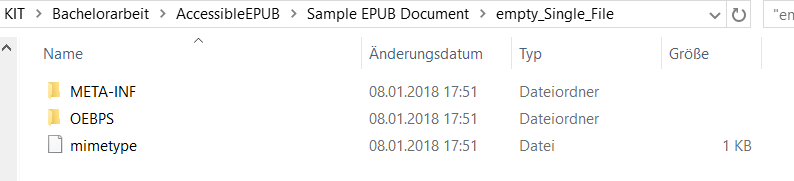
\includegraphics[width=\linewidth]{figures/epubFolderStructure.png}
	\caption{Folder structure within an EPUB file}
	\label{fig:epubFolderStructure}
\end{figure}

\subsection{Changes from EPUB 2 to EPUB 3 and EPUB 3.1}

The EPUB working group has also made some important changes from EPUB 2 to EPUB 3  to make it more accessible. Equations can now be displayed in MathML.\cite{EPUB30changes} In EPUB 2 they had to either be displayed in normal XHTML or as images. It is difficult towrite math in normal XHTML, as complex symbols like fractions, roots and plus-minus might not be displayed properly. Images can display the equations properly, but only if they are SVG files can they scaled without quality loss. Furthermore, all images are not as accessible as MathML, which can be scaled properly and can be read by a screen reader.

In EPUB 2 the navigation was done with a NCX file, usually named \lstinline|toc.ncx|.\cite{EPUB3bp} In EPUB 3 this is now done instead with a XHTML file, and can be created with regular XHTML elements like \lstinline|ol| and \lstinline|ul|, for ordered and unordered lists, respectively. XHTML is much more widely used and is already an important format in EPUB 3, while NCX files have a distinct syntax, which has to be learned in addition to XHTML. Replacing NCX means that the creator has one less document format to worry about.

Scripting with JavaScript with strongly discouraged in EPUB 2, but in EPUB 3 it is optional.\cite{EPUB3bp} This allows documents to be interactive, but it is recommended that information is not hidden if a device does not support scripting. This should be done with a process called progressive enhancement. In essence, content should first be designed in the most accessible way, and then layers of enhancement should be added, which might not be supported on all devices. For example, if the creator wants to add an animation with JavaScript to the document, it might be better to add several images showing the stills of the animation at important junctions. Each still image would also have alternative text for users with screen readers. The creator could then add an animation for devices that support it, enhancing their experience.

EPUB 2 supports Cascading Style Sheets(CSS) 2, while EPUB 3 supports CSS 2.1 with added modules from CSS 3 which were defined as basic EPUB CSS Profile. The EPUB CSS Profile was removed in EPUB 3.1 and the IDPF defined more general CSS support requirements in its place.\cite{EPUB31changes} Henceforth they also use the more general definition of CSS as mentioned by CSS Working Group, which results in creators not being required to learn specific CSS attributes only seen in EPUB.

One new feature in EPUB 3 is media overlays, which might be of considerable interest to people with accessibility requirements.\cite{EPUB3bp} This feature is supposed help integrate Digital Accessible Information System (DAISY) digital talking books in EPUB 3. The first DAISY Standard originated in Sweden in 1994. DAISY is a digital standard to create an audio substitute for printed media.\cite{daisyAccessibility} When it was created the primary audio media were tapes and CDs, both with rather limited runtime. Discs with DAISY books, however, can hold 40 hours of audio, while the corresponding number for CDs is about 74 minutes.\cite{wasIstDaisy} DAISY books also allow the user to skip between chapters, pages or even sentences and create bookmarks. EPUB 3 has the same features, but media overlays now allow it to synchronize audio narration to text. The user can still use Text-To-Speech(TTS) rendering, but as it is computer generated, it might not pronounce all words properly. Prerecorded audio narration is of course better at this, and now the user can switch between reading and audio narration without navigating in an audio file.

However, many of these changes are not supported by reading devices, and this will be topic of discussion in chapter \ref{ch:Evaluation EPUB Standard}, where reading devices are evaluated, both software and hardware.\cite{EPUB30changes} 


\subsection{EPUB Structure}
The first step to knowing what an EPUB is by knowing what an EPUB file is. It has the extension \lstinline{.epub}, but is actually just a renamed ZIP file(extension \lstinline{.zip}). After the extension of the EPUB file is changed, the new ZIP file can be decompressed and the files within the document can be accessed.\cite{EPUB3bp}

Compressing the folder back to a ZIP file has to be done with care. The mimetype should be the first file to added to the ZIP container and not the other two folders. If this is not done properly, the EPUB file is not in the proper format and some readers can not read the file.


\begin{figure}
	\begin{lstlisting}
	application/epub+zip
	\end{lstlisting}
	\caption{Contents of the \lstinline{mimetype} file}
	\label{fig:mimetype}
\end{figure}

The folder structure of an EPUB file is shown in figure~\ref{fig:epubFolderStructure}. The file named \lstinline{mimetype} has a single line indicating that the ZIP file contains an EPUB. The META-INF folder contains just one file named \lstinline{container.xml}. This file has to indicate the location of the package file(extension \lstinline{.opf}). The name of the folder named OEBPS can actually be freely chosen, however, \lstinline{container.xml} has to describe the path to the package file correctly. OEBPS stands for Open eBook Publication Structure, which was the format superseded by EPUB.\cite{OPSspecs} 

\begin{figure}
	\begin{lstlisting}
	<?xml version="1.0" encoding="UTF-8"?>
	<container xmlns="urn:oasis:names:tc:opendocument:xmlns:container" version="1.0">
	<rootfiles>
	<rootfile full-path="EPUB/package.opf" media-type="application/oebps-package+xml"/>
	</rootfiles>
	</container>
	
	\end{lstlisting}
	\caption{Contents of container.xml}
	\label{fig:containerXML}
\end{figure}

\subsubsection{Package document}

The OEBPS folder traditionally contains the package document which has the extension \lstinline{.opf}. The package document contains five XML declarations:

\begin{itemize}
	\item \lstinline{metadata} (required)
	\item \lstinline{manifest} (required)
	\item \lstinline{spine} (required)
	\item \lstinline{guide} (optional)
	\item \lstinline{bindings}. (optional)
\end{itemize}

The \lstinline{metadata} declaration information about the document in Dublin Core form. Only \lstinline{dc:title, dc:language, dc:identifier} and one \lstinline{meta} are required, but there are several optional ones. The data entries have to follow the specifications. 

\begin{figure}
	\begin{lstlisting}
	<metadata xmlns:dc="http://purl.org/dc/elements/1.1/" xmlns:opf="http://www.idpf.org/2007/opf" xmlns:dcterms="http://purl.org/dc/terms/">
		<dc:title>BookTitle</dc:title>
		<dc:creator>Author</dc:creator>
		<dc:language>en</dc:language>
		<dc:publisher>Publisher</dc:publisher>
		<dc:identifier id="BookId">BookIdentificationNumber</dc:identifier>
		<meta property="dcterms:modified">2018-02-07T10:43:33Z</meta>
		<meta name="AccessibleEPUB" content="0.1.0" />
	</metadata>
	\end{lstlisting}
	\caption{The various Dublin Core tags in the \lstinline{metadata}}
	\label{fig:metadata}
\end{figure}

The \lstinline{manifest} declarations contains all of the files which should be included in the EPUB file with an ID, the path to each file and an appropriate declaration of the media type.  Properties also have to entered. If a \lstinline{XHTML} file is a navigation document, \lstinline{nav} has to be entered in the properties.

\begin{figure}
	\begin{lstlisting}
	<manifest>
		<item id="ncx" href="toc.ncx" media-type="application/x-dtbncx+xml"/>
		<item id="Content.xhtml" href="Text/Content.xhtml" media-type="application/xhtml+xml"/>
		<item id="style.css" href="Styles/style.css" media-type="text/css"/>
		<item id="navid" href="Text/nav.xhtml" media-type="application/xhtml+xml" properties="nav"/>
	</manifest>
	\end{lstlisting}
	\caption{Files listed in the \lstinline{manifest}}
	\label{fig:manifest}
\end{figure}

The \lstinline{spine} declares the default reading order of the EPUB. The reader is free to go to whatever page they want, but the \lstinline|spine| allows the document creator to set a logical order of the files in the spine. The only file types which do not require a fallback in the \lstinline|spine| are XHTML and SVG files.\cite{EPUB3bp} 

\begin{figure}
	\begin{lstlisting}
	<spine toc="ncx">
		<itemref idref="Content.xhtml"/>
	</spine>
	\end{lstlisting}
	\caption{The reading order declared in the \lstinline{spine}}
	\label{fig:spine}
\end{figure}

The \lstinline|guide| is deprecated and only needed for EPUB 2, but it is useful for backwards compatibility. \lstinline|bindings| is used for fallback options for interactive media. Both of these are optional and will therefore not be discussed further in this bachelor thesis.

\subsubsection{Navigation}

The OEBPS folder also contains a file, normally named nav.xhtml, which is the table of contents. The table of contents can be used to navigate to any tagged section and is created by simply making an ordered or unordered list in HTML. A short example is shown in figure~\ref{fig:tableOfContents}. 

\begin{figure}
	\begin{lstlisting}
	<nav epub:type="toc" id="toc">
	<h1>Table of Contents</h1>
		<ol>
			<li>
			<a href="../Text/Content.xhtml">Start</a>
			</li>
		</ol>
	</nav>		
	\end{lstlisting}
	\caption{An example table of contents}
	\label{fig:tableOfContents}
\end{figure}

\subsubsection{Content documents}

One of the primary documents of an EPUB document are Extensible Hypertext Markup Language (XHTML) file. XHTML is used, because they are formats of the web. Websites have to be displayed on a variety of devices, from phones with screen dimensions of a few inches to 50 inch television screens with varying display resolutions. The content is therefore reflowable and suits Ebook readers as they are available in various sizes. 

Another primary document of EPUB documents are Scalable Vector Graphics (SVG) files. They are based on XML and while image formats like JPEG and PNG are raster based with pixels, SVG files are vector based and are rendered with mathematical formulas. This means that they retain their appearance at any size and do not get blurry at larger sizes than they created at.


\subsection{Goal of this thesis}

The goals of this thesis will be described in the following sections.

\begin{enumerate}
	\item Create an accessible document standard based on EPUB 3
	\item Develop an editor which will then be able to create EPUB files of this new standard.
\end{enumerate}

\subsubsection{Document standard}
The first goal of this thesis is to create an document standard based on EPUB 3. This document standard must also include support for STEM (Science, Technology, Engineering, Mathematics) subjects. Existing literature, both electronic and in paper form, is frequently not accessible due to the figures and mathematical formulas in them. If the figure does not have proper captions or alternative text, blind people will be unable to extract the knowledge sighted people will from it. Blind people read formulas with specialized mathematical braille notation, such as Nemeth code in the USA and Marburger mathematical code in Germany.\cite{augenbitWiki} However, few books are printed in braille, braille printers are uncommon and expensive and the resulting books tend to be very heavy. When the textbooks are in electronic form, the mathematical equations have to written in LaTeX code. The quadratic equation is shown in figure~\ref{fig:quadEquaPng}, while the corresponding LaTeX code is shown in figure~\ref{fig:quadEquaLatex}. Visually impaired people have different requirement for mathematics and graphics. They should scale and not get pixelated when the size in increased, as shown in figure This is best done with SVGs, which were mentioned in last chapter. Visually impaired people also need the text to be a sans-serif font, like Helvetica or Arial.\cite{pdfBarrierefrei}

\begin{figure}
	\begin{center}
	
\includegraphics[width=\linewidth/3]{figures/QuadraticEquation.png}
	\end{center}
	\caption{Quadratic Equation}
	\label{fig:quadEquaPng}
\end{figure}

\begin{figure}
	\begin{lstlisting}
	{x = \frac{ - b \pm \sqrt {b^2 - 4ac}}{2a}}
	\end{lstlisting}
	\caption{Quadratic Equation in LaTeX code}
	\label{fig:quadEquaLatex}
\end{figure}

\begin{figure}
	\begin{center}
		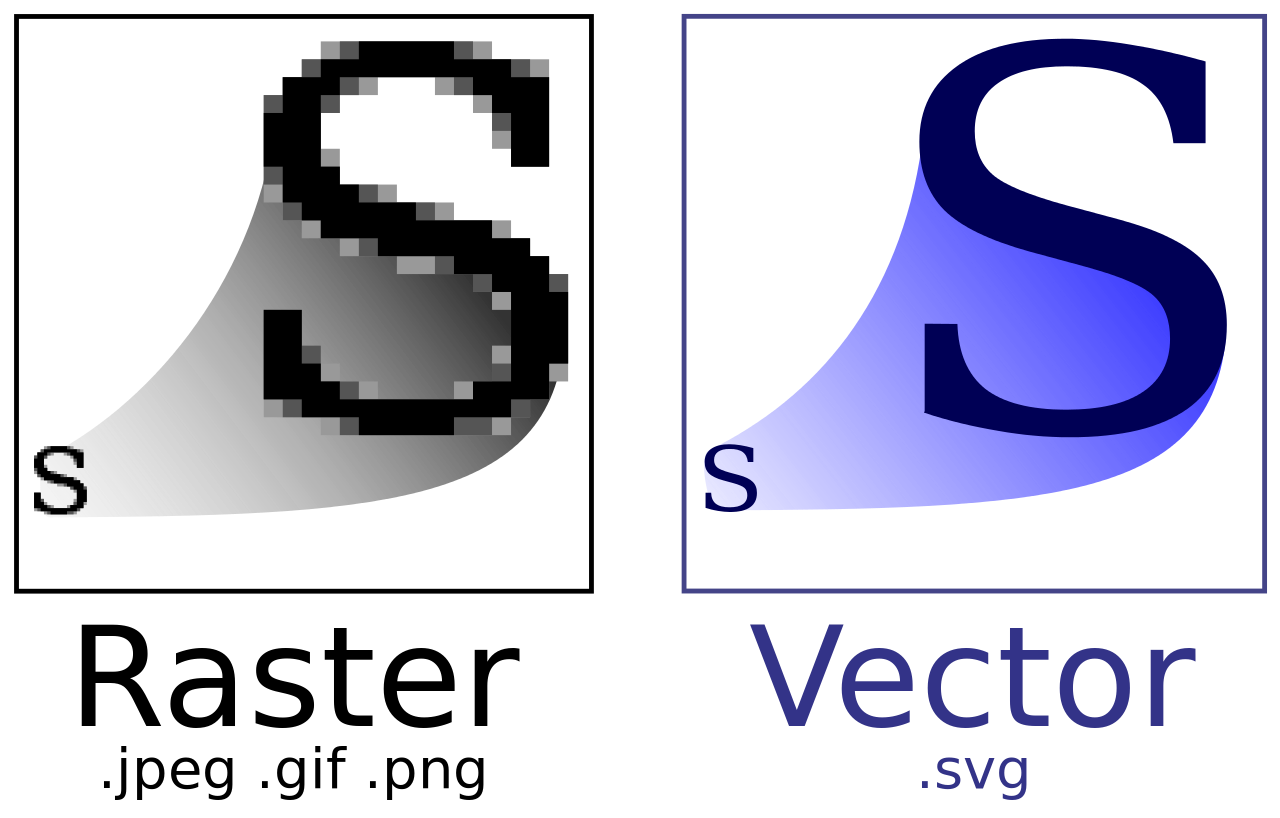
\includegraphics[width=\linewidth/2]{figures/bitmapVsSvg.png}
	\end{center}
	
	\caption{$Source: https://upload.wikimedia.org/wikipedia/commons/thumb/\\6/6b/Bitmap_VS_SVG.svg/1280px-Bitmap_VS_SVG.svg.png$}
	\label{fig:bitmapSvg}
\end{figure}

Sighted people have their formulas appear as a serif font as shown in figure \ref{fig:quadEquaPng}, visually impaired people need it to appear as sans-serif and blind people needs LaTeX code.\cite{augenbitWiki} This is difficult to do in one document, so separate documents have to be created for the blind and the visually impaired, creating additional work for the document creator. The new standard must have all include versions for sighted, visually impaired and blind people in one document to simplify the creation process. Instead of using the currently dominant formats, PDFs and word documents, this will be done with EPUB 3, because they are more suited to electronic formats and allow dynamic content, thanks to CSS 3 and JavaScript. There will be a easy way to switch between three versions. For example, when the blind version is chosen, content such as formulas will change to LaTeX code.

\subsubsection{Editor}
The second goal of this thesis is to develop an editor to create documents of this standard easily. It should not require programming ability and allow insertion of formulas and figures which will be available in all three versions. The editor should not be difficult to learn and be  What-You-See-Is-What-You-Get(WYSIWYG), much like a word processor, instead of XHTML which requires coding.